% Декомпозиция поверхностной сетки.
\subsection{Декомпозиция поверхностной неструктурированной расчетной сетки для масштабирования вычислений на суперкомпьютере}

\subsubsection{Описание методов декомпозиции}

Все описанные в работе алгоритмы декомпозиции рассматриваются на примере тестовой трехмерной поверхностной сетки (wing), состоящей из ячеек-треугольников.
Сетка представляет собой профиль крыла летательного аппарата и содержит 9900 узлов, 29205 ребер и 19306 ячеек.
Внешний вид тестовой расчетной сетки представлен на рис. 2.
Данный трехмерный профиль был сгенерирован из двумерного профиля NACA 0012.

\begin{figure}[ht]
	\centering
		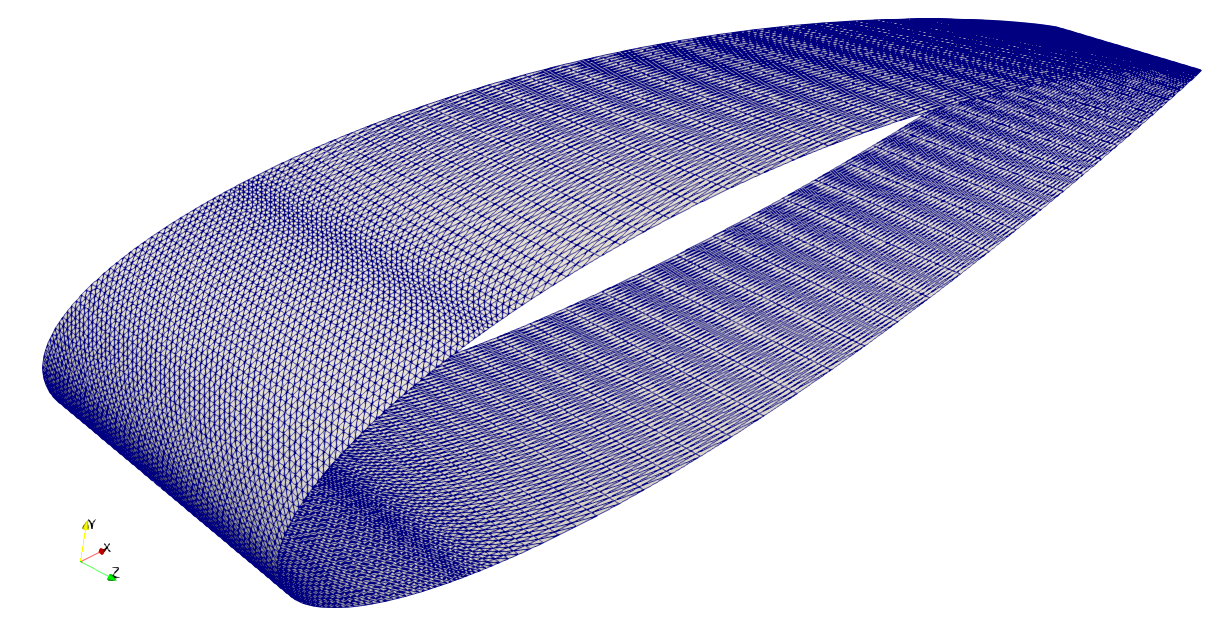
\includegraphics[width=0.6\textwidth]{./pics/text_2_decompsurf/wing_grid.png}
	\caption{Внешний вид расчетной сетки wing, используемой для тестирования алгоритмов декомпозиции.}
	\label{fig:text_2_decompsurf_wing_grid}
\end{figure}

В качестве первого и самого простого алгоритма декомпозиции представим алгоритм случайного распределения ячеек расчетной сетки по доменам.
Результат применения данного алгоритма к тестовой сетке показан на рис. 3.
Данный алгоритм имеет достаточно низкое значение по критерию $D$, то есть распределение ячеек по доменам равномерное, однако при случайном распределении практически все ребра с высокой долей вероятности являются междоменными, что порождает огромный объем данных, которыми нужно обмениваться при синхронизации вычислений.
Также следует отменить, что при случайном распределении ячеек по доменам любые два домена оказываются соседними, граф связности доменов является полным.
Таким образом, каждый домен должен обмениваться данными со всеми остальными доменами по достаточно протяженным границам.
Также данный алгоритм становится совершенно непригодным, когда возникает необходимость создания в доменах буферных зон вблизи границ с глубиной больше единицы.
Использование таких буферных зон может потребоваться для реализации численных методов повышенной точности.

На данном этапе уместно будет упомянуть механизм частичного сокрытия издержек на обмены данными за основными вычислениями.
Данный механизм описан в [15].
Все ячейки каждого домена можно разделить на внутренние и граничные.
Внутренние ячейки домена -- ячейки, все соседи которых также принадлежат тому же домену.
Граничные ячейки -- это все остальные ячейки. Ценность внутренних ячеек состоит в том, что они не участвуют в обменах данными с соседними доменами (если не используются разностные схемы с повышенным порядком точности), поэтому обработку внутренних ячеек на следующей итерации расчетов можно начинать, не дожидаясь завершения обменов данными на ребрах, составляющих границу между доменами.
Понятно, что данный подход неприменим при использовании случайного распределения ячеек по доменам, так как в большинстве случаев множества внутренних ячеек доменов оказываются практически пустыми.

\begin{figure}[ht]
	\centering
		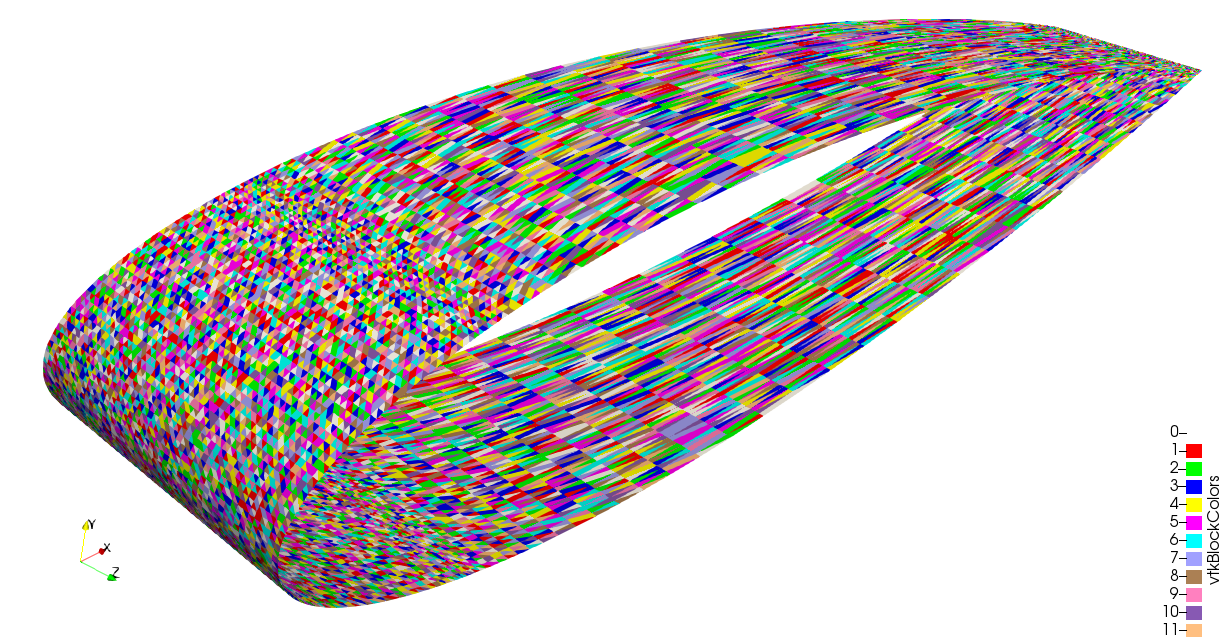
\includegraphics[width=0.6\textwidth]{./pics/text_2_decompsurf/wing_random_32.png}
	\caption{Результат декомпозиции расчетной сетки на 32 домена с помощью случайного распределения ячеек по доменам.}
	\label{fig:text_2_decompsurf_wing_random_32}
\end{figure}

Рассмотрим семейство алгоритмов декомпозиции, в которых учитываются только индексы распределяемых ячеек и никак не учитываются другие их данные.
Под индексом в данном случае понимается номер ячейки в общем массиве ячеек расчетной сетки.
Уже по этому факту становится понятно, что такие алгоритмы не могут претендовать на высокое качество, так как их результат существенным образом зависит просто от порядка хранения данных расчетной сетки.
Самым простым из алгоритмов данного класса является алгоритм линейного распределения ячеек по доменам.
Так как в каждый домен в среднем должно войти по $\frac{S}{n}$ ячеек (для простоты не будем обращать внимание на то, что это число может быть нецелым), то можно ячейки с номерами из диапазона $[0, \frac{S}{n} - 1]$ отнести к первому домену, ячейки с номерами $[\frac{S}{n}, 2\frac{S}{n} - 1]$ ко второму домену и так далее.
При такой декомпозиции, конечно, можно добиться равномерного распределения ячеек по доменам, однако значения параметров $I$ и $L$ в общем случае предугадать невозможно.
Например, на рассматриваемой тестовой сетке видно, что деление на домены вдоль профиля крыла (как это показано на рис. 4) порождает очень длинные границы между соседними доменами.
Было бы гораздо эффективнее производить деление сетки поперек профиля.

\begin{figure}[ht]
	\centering
		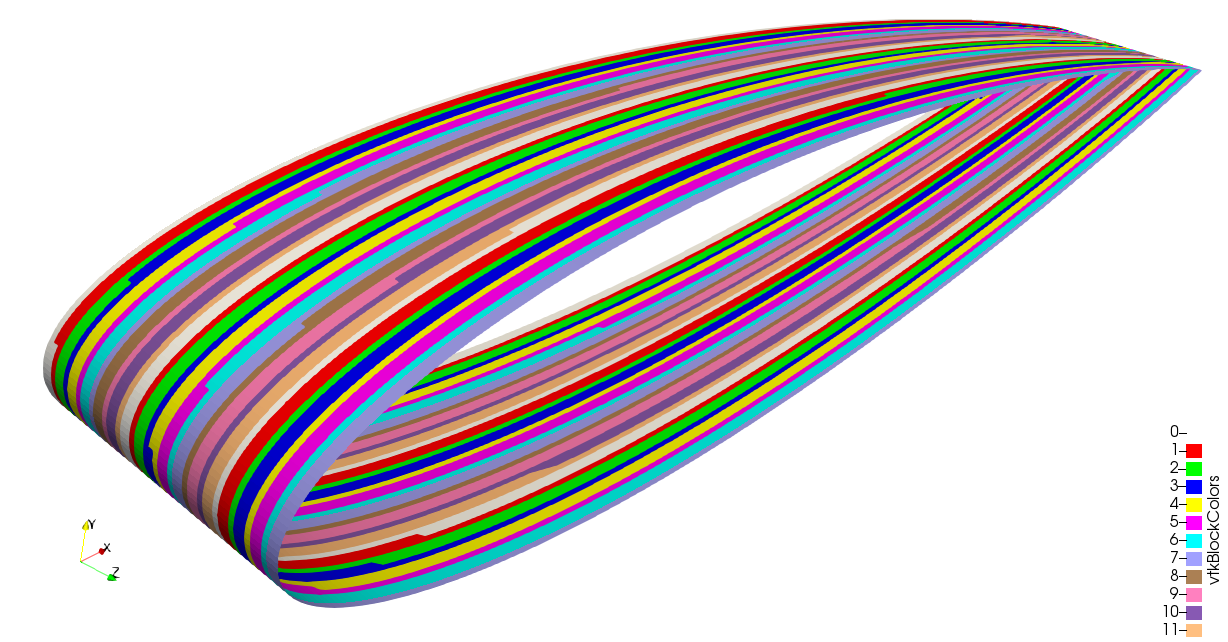
\includegraphics[width=0.6\textwidth]{./pics/text_2_decompsurf/wing_linear_32.png}
	\caption{Результат декомпозиции расчетной сетки на 32 домена с помощью линейного разделения множества индексов ячеек.}
	\label{fig:text_2_decompsurf_wing_linear_32}
\end{figure}

В общем случае ячейки с непрерывным диапазоном индексов не обязаны составлять не то что компактные домены с границами небольшой протяженности, а вообще могут порождать несвязные домены, с артефактами, выколотыми ячейками и так далее.
Применение таких алгоритмов оправдано только при обладании некоторой априорной информацией о структуре расчетной сетки (например, если известно, что сетка на самом деле является блочно-структурированной, в которой отдельные блоки соответствуют непрерывным диапазонам индексов ячеек).

Большой класс алгоритмов формируется из так называемых алгоритмов наращивания доменов.
В основе данных алгоритмов лежит следующий принцип: вначале выбирается ячейка (или несколько ячеек), от которой далее производится наращивание домена путем последовательного добавления к ней соседних ячеек.
В рамках данного класса алгоритмов при последовательном создании доменов размера $\frac{S}{n}$ получим жадный алгоритм Фархата, результатом которого являются домены с очень протяженными границами [16].
При использовании одновременного роста сразу нескольких доменов от случайных ячеек расчетной сетки получаем алгоритм пузырькового роста [17], который требуется запускать на расчетной сетке итерационно несколько раз для получения приемлемых характеристик качества разбиения.
При этом алгоритм пузырькового роста не гарантирует сбалансированного разбиения ячеек сетки по доменам (для достижения этого необходимо производить дополнительную коррекцию).
Также следует отметить инкрементальный алгоритм декомпозиции графов [18], особенностью которого является возможность освобождения части ячеек, уже распределенных по доменам, с последующим повторением роста доменов.

Мы в данном случае рассматриваем простой алгоритм наращивания доменов, в котором все домены наращиваются одновременно, начиная с некоторых случайно выбранных ячеек сетки.
При этом поддерживается связность доменов -- если в какой-то момент домену больше некуда расти, то он прекращает свое наращивание и больше не расширяется.
Таким образом, возможно генерация крайне неравномерных по количеству ячеек доменов. Пример результата применения описанного алгоритма приведен на рис. 5.

\begin{figure}[ht]
	\centering
		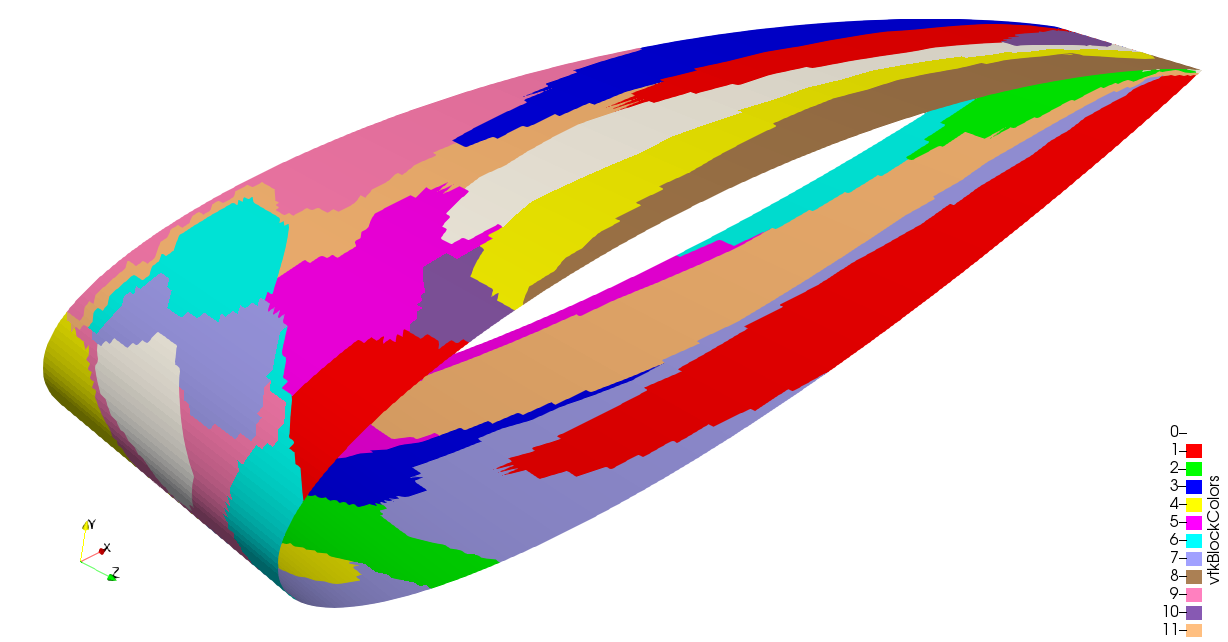
\includegraphics[width=0.6\textwidth]{./pics/text_2_decompsurf/wing_rgrow_32.png}
	\caption{Результат декомпозиции расчетной сетки на 32 домена с помощью алгоритма наращивания доменов от случайных ячеек.}
	\label{fig:text_2_decompsurf_wing_rgrow_32}
\end{figure}

Кроме приведенных алгоритмов существует еще большое количество подходов к декомпозиции расчетных сеток, среди них алгоритмы, основанные на методе спектральной бисекции [19], диффузионные и генетические алгоритмы [20], иерархические алгоритмы [21] и многие другие.
Наиболее полный обзор различных алгоритмов декомпозиции расчетных сеток можно найти в [22] и [23].
Большинство из существующих алгоритмов декомпозиции либо не достаточно полно удовлетворяют критериям качества декомпозиции, либо должны выполняться итерационно, требуют локального уточнения и других корректирующих действий, что требует существенного вычислительного времени.

Возникает потребность создания простого быстрого алгоритма декомпозиции поверхностной неструктурированной расчетной сетки, в результате которого формируются связные домены с границами малой протяженности между ними.

\subsubsection{Иерархический метод декомпозиции с выбором наилучшего разбиения}

В работе [22] описан параллельный алгоритм геометрической декомпозиции сеточных данных.
Во время работы данного алгоритма происходит последовательное деление текущего домена пополам с помощью сечения плоскостью.
На рис. 6. продемонстрирована схема, по которой изначальный головной домен h делится на пару доменов hl (left), hr (right), каждый из которых делится далее пополам и так далее на любое количество доменов, равное степени двойки.

\begin{figure}[ht]
	\centering
		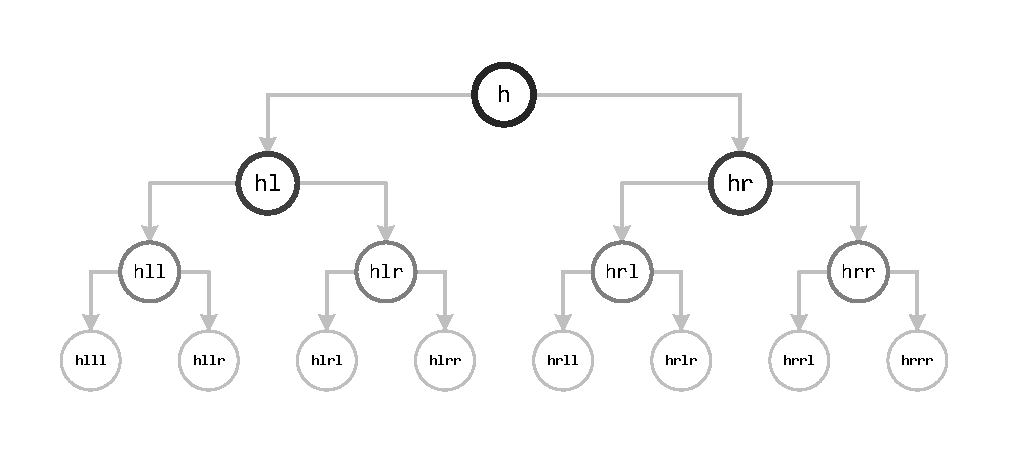
\includegraphics[width=1.0\textwidth]{./pics/text_2_decompsurf/hierarchical.pdf}
	\caption{Иллюстрация иерархического трехуровневого разделения головного домена.}
	\label{fig:text_2_decompsurf_hierarchical}
\end{figure}

Данный алгоритм предлагается расширить, введя в него произвольные критерии разбиения текущего домена на пару более мелких доменов.
Вначале рассмотрим схему простого деления домена пополам с использованием произвольного признака, по которому производится деление (см. рис. 7).

\begin{figure}[ht]
	\centering
		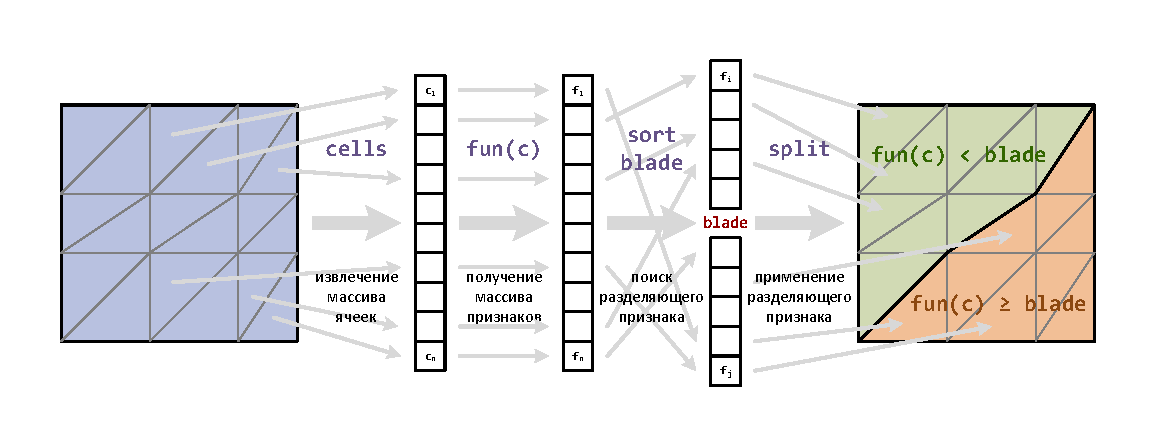
\includegraphics[width=1.0\textwidth]{./pics/text_2_decompsurf/split.pdf}
	\caption{Схема выполнения разделения домена пополам по заданному признаку fun.}
	\label{fig:text_2_decompsurf_split}
\end{figure}

Будем описывать алгоритм разделения домена на две части в нотации языка Python.
Пусть задан массив ячеек домена (h - head) и произвольная функция извлечения признака из ячейки (fun).
Первым шагом является вычисление массива признаков для всех ячеек (s - signs): s = list(map(fun, h)).
После получения массива признаков его нужно отсортировать: s.sort().
В отсортированном массиве признаков следует выбрать среднее значение (b - blade): b = s[len(s) // 2].
Данное значение будет использоваться для разделения домена на два мелких домена (hl - head left, hr - head right) с помощью применения двух простых фильтров: hl, hr = list(filter(h, lambda x: fun(x) < b)), list(filter(h, lambda x: fun(x) >= b)).

После разделения домена на два более мелких домена можно вычислить параметр, отражающий эффективность разбиения.
В качестве такого параметра предлагается использовать длину границы между двумя образованными новыми доменами.
Таким образом, критерий разбиения зависит от функции вычисления признака (fun).
В свою очередь это означает, что при выполнении разбиения не обязательно ограничиваться одной функцией вычисления признака, вместо этого можно подать список функций, для каждой функции вычислитель показатель качества разбиения и в результате остановиться на той функции вычисления признака, которая в конечном итоге приводит к наиболее эффективному разбиению.
Если в качестве функций вычисления признака ячейки использовать просто извлечение трех координат центров ячеек, то мы получим в чистом виде алгоритм геометрической декомпозиции сетки с выбором для дробления наиболее протяженного размера по одной из координат.
Результат применения данного алгоритма показан на рис. 8.

\begin{figure}[ht]
	\centering
		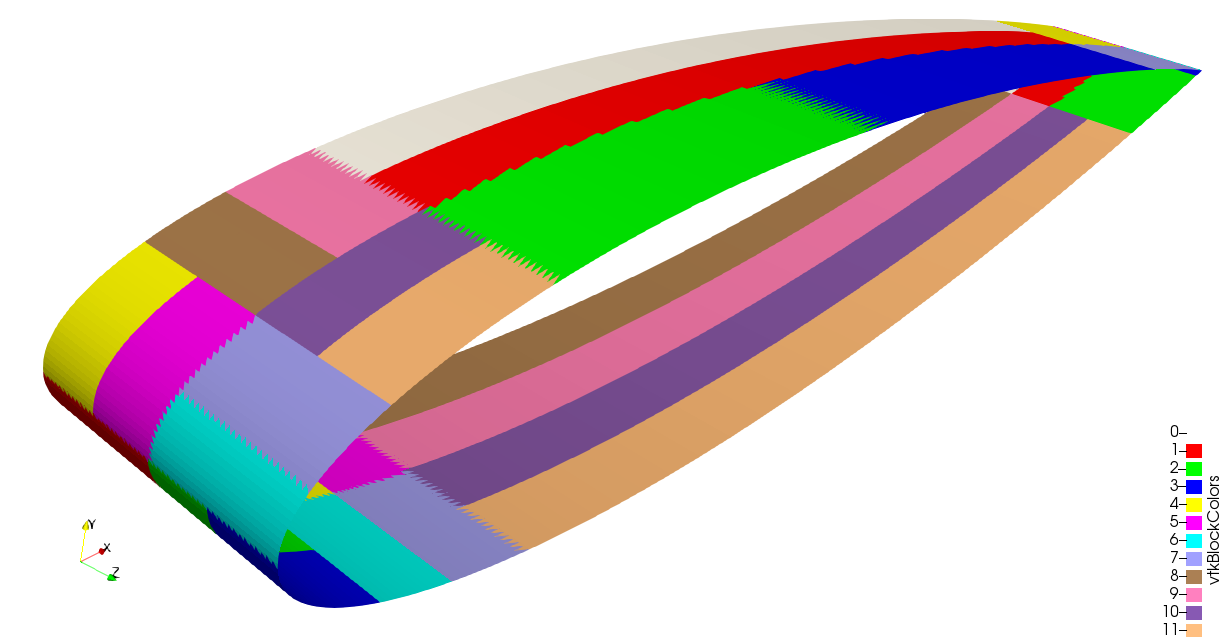
\includegraphics[width=0.6\textwidth]{./pics/text_2_decompsurf/wing_hierarchical_32.png}
	\caption{Результат декомпозиции расчетной сетки на 32 домена с помощью иерархического алгоритма.}
	\label{fig:text_2_decompsurf_wing_hierarchical_32}
\end{figure}

Варьируя набор функций вычисления признаков, по которым можно выполнять разбиение домена, возможно выполнять геометрическую декомпозицию вдоль направления любой кривой, для которой вычисляется проекция ячейки.
Декомпозиция с помощью данного метода не ограничивается только геометрическими признаками.
Функции вычисления признаков могут использоваться для анализа физических данных ячеек, например, для локализации и выделении в отдельные домены областей с повышенным давлением.

В рамках данной работы описанный алгоритм декомпозиции поверхностной неструктурированной расчетной сетки применялся к поверхностным сеткам, используемым для расчета обледенения поверхности летательного аппарата [24,25].
При расчете обледенения летательного аппарата основной объем вычислений относится к обработке поверхностных ячеек, общие данные между соседними доменами собраны на междоменных ребрах, что обеспечивает небольшой обмен данных, которыми требуется обмениваться в ходе синхронизации вычислений.
Характерный размер таких сеток составил около $10^5$ ячеек, рассматривались как односвязные, так и многосвязные поверхности, а также поверхности, состоящие из нескольких изолированных друг от друга зон.

\subsubsection{Результаты экспериментов}

На рисунках 9-11 представлены графики параметров $D$, $I$, $L$, вычисленные во время применения к тествой сетке wing различных алгоритмов декомпозиции поверхностной расчетной сетки на разное количество доменов от 2 до 32.
На данных графиках введены следующие кратные названия алгоритмов: random -- случайное распределение ячеек по доменам, linear -- линейное разделение ячеек между доменами по индексу, rgrow -- алгоритм наращивания доменов от случайных ячеек, hierarchical -- иерархическое деление доменов пополам по одной из трех координат (в качестве функций вычисления признаков ячеек брались просто функции извлечения каждой из трех координат центра ячейки).

\begin{figure}[ht]
	\centering
		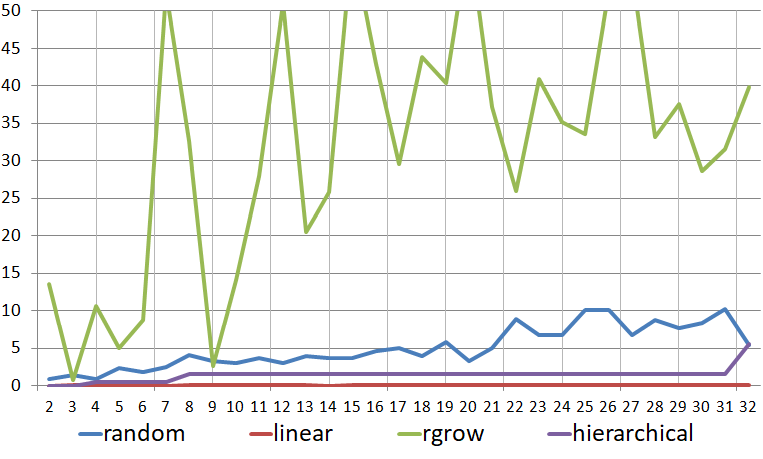
\includegraphics[width=0.6\textwidth]{./pics/text_2_decompsurf/wing_50_blocks_dev.png}
	\caption{Графики отклонения максимального размера домена от оптимального значения (в процентах) для расчетной сетки wing при разных алгоритмах декомпозиции.}
	\label{fig:text_2_decompsurf_wing_50_blocks_dev}
\end{figure}

\begin{figure}[ht]
	\centering
		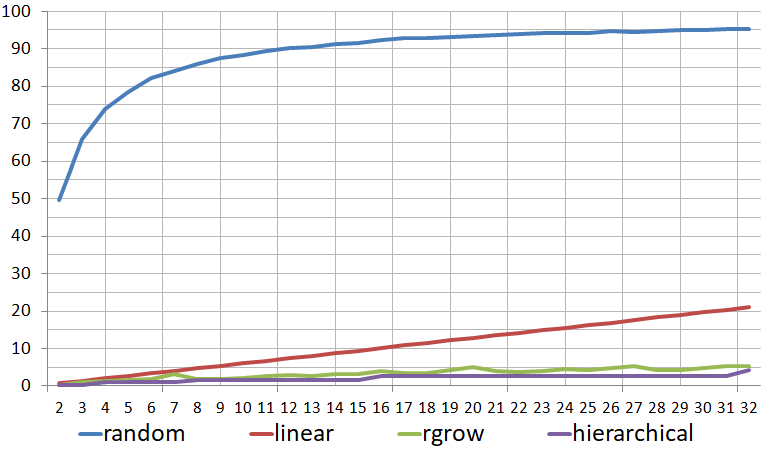
\includegraphics[width=0.6\textwidth]{./pics/text_2_decompsurf/wing_50_inter_edges.png}
	\caption{Графики доли (в процентах) количества ребер, являющихся границей между разными доменами, от общего количества ребер расчетной сетки wing при разных алгоритмах декомпозиции.}
	\label{fig:text_2_decompsurf_wing_50_inter_edges}
\end{figure}

\begin{figure}[ht]
	\centering
		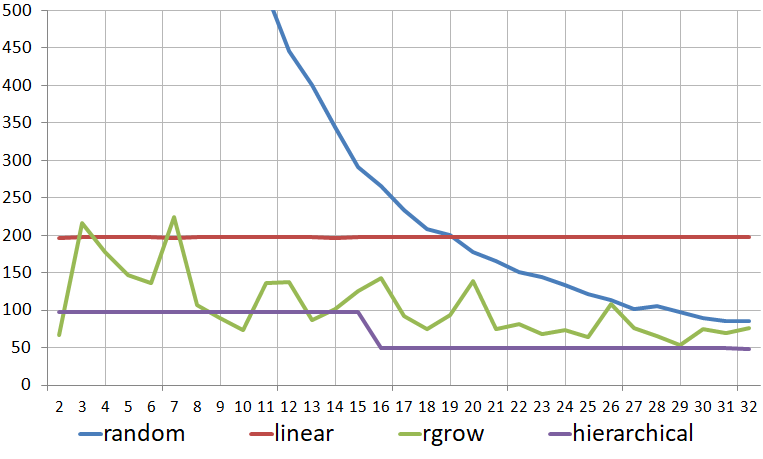
\includegraphics[width=0.6\textwidth]{./pics/text_2_decompsurf/wing_50_max_border.png}
	\caption{Графики максимальной длины границы между доменами при декомпозиции расчетной сетки wing с помощью разных алгоритмов декомпозиции.}
	\label{fig:text_2_decompsurf_wing_50_max_border}
\end{figure}

При этом отметим, что при использовании алгоритма rgrow умышленно использовалась только одна итерации наращивания, для демонстрации того, насколько неравномерным может быть распределение размеров доменов при случайном выборе стартовых ячеек (из рис. 9 видно, что отклонение может достигать 50\% и более).

На рисунках 12-14 приведены аналогичные графики параметров $D$, $I$, $L$, полученные на сетке, более приближенной к реальной геометрии летательного аппарата (сетка ref). Данная сетка обладает следующими характеристиками: количество узлов -- 228722, количество ребер -- 685192, количество поверхностных ячеек -- 456469.

\begin{figure}[ht]
	\centering
		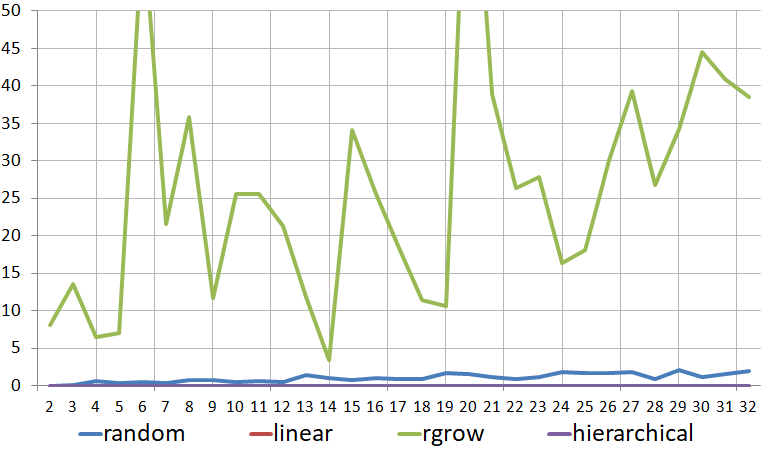
\includegraphics[width=0.6\textwidth]{./pics/text_2_decompsurf/air_inlet_blocks_dev.png}
	\caption{Графики отклонения максимального размера домена от оптимального значения (в процентах) для расчетной сетки ref при разных алгоритмах декомпозиции.}
	\label{fig:text_2_decompsurf_air_inlet_blocks_dev}
\end{figure}

\begin{figure}[ht]
	\centering
		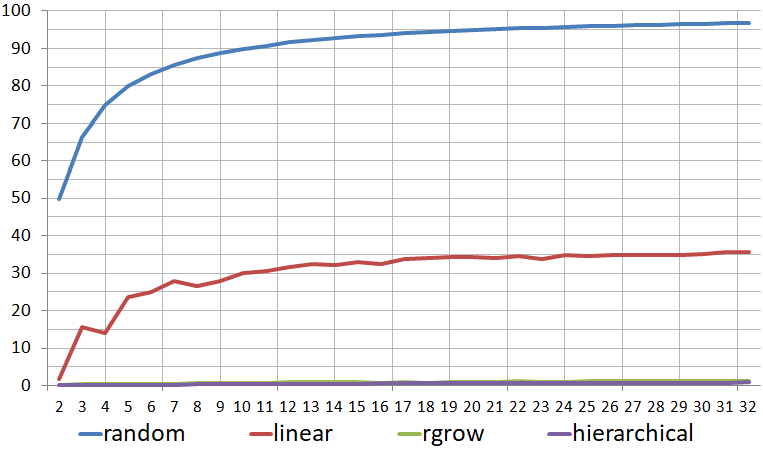
\includegraphics[width=0.6\textwidth]{./pics/text_2_decompsurf/air_inlet_inter_edges.png}
	\caption{Графики доли (в процентах) количества ребер, являющихся границей между разными доменами, от общего количества ребер расчетной сетки ref при разных алгоритмах декомпозиции.}
	\label{fig:text_2_decompsurf_air_inlet_inter_edges}
\end{figure}

\begin{figure}[ht]
	\centering
		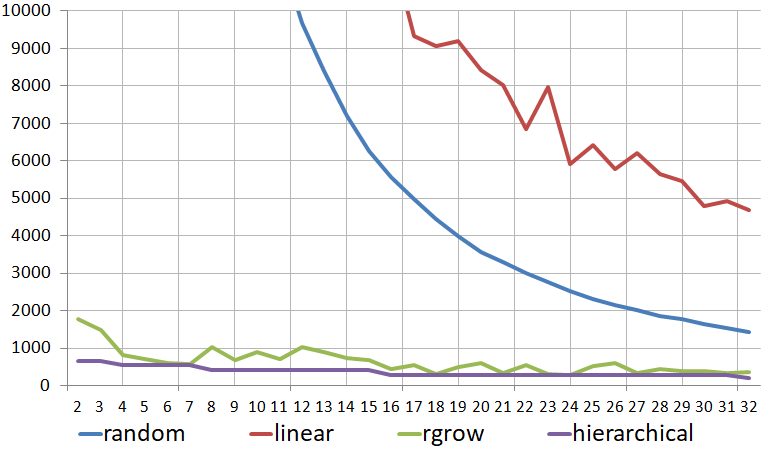
\includegraphics[width=0.6\textwidth]{./pics/text_2_decompsurf/air_inlet_max_border.png}
	\caption{Графики максимальной длины границы между доменами при декомпозиции расчетной сетки ref с помощью разных алгоритмов декомпозиции.}
	\label{fig:text_2_decompsurf_air_inlet_max_border}
\end{figure}

Из приведенных графиков можно сделать выводы, что из представленных алгоритмов иерархическое деление доменов с выбором оптимального критерия деления из списка функций вычисления признаков ячеек является наиболее приемлемым по параметрам $D$, $I$, $L$, то есть с помощью данного алгоритма генерируется достаточно равномерное распределение ячеек по доменам при низкой общей доле междоменных ребер и малой протяженности границ между доменами.
Отметим также, что наиболее затратной операцией с точки зрения асимптотики при разделения доменов является сортировка признаков ячеек, что с учетом иерархии дробления доменов приводит к сложности всего алгоритма не хуже $n \cdot log^2 n$.

В ходе выполнения работы рассмотрен ряд алгоритмов декомпозиции поверхностной неструктурированной расчетной сетки и проведен анализ эффективности этих алгоритмов по следующим параметрам: максимальное отклонение размера получившегося домена от идеального значения, доля междоменных ребер в итоговом разбиении, протяженность наиболее длинной границы между доменами.
Предложен алгоритм иерархического разбиения доменов расчетной сетки с помощью выбора оптимального критерия разбиения на основе списка функций получения признаков ячеек.
Полученные характеристики предложенного алгоритма, простота реализации и скорость его работы позволили использовать данный алгоритм в промышленных программных кодах для декомпозиции поверхностных расчетных сеток с целью улучшения масштабируемости суперкомпьютерных расчетов.
